\documentclass[twocolumn,10pt]{article}

\usepackage[top=2cm,bottom=2cm,left=1.5cm,right=1.5cm]{geometry}

\usepackage{lipsum}

\usepackage{abstract}
\renewcommand{\abstractnamefont}{\normalfont\normalsize\bfseries}
\renewcommand{\abstracttextfont}{\normalfont\small}
\setlength{\absleftindent}{1em}
\setlength{\absrightindent}{2em}

\usepackage{titlesec}
\titleformat{\section}[block]{\Large\bfseries\filcenter}{}{}{}
% \titleformat{\subsection}[block]{\large\bfseries\filcenter}{}{}{}

\usepackage[dvipsnames]{xcolor}
\usepackage[
    colorlinks=true,
    allcolors=blue % Feel free to change the colour if you prefer another :)
]{hyperref}
\usepackage[
    backend=biber,
    style=numeric-comp,
    sortcites=true,
    giveninits=true,
    hyperref=true,
    sorting=nyt,
    natbib=true,
]{biblatex}
\addbibresource{references.bib}
\renewcommand*{\bibfont}{\footnotesize}
% Get the citations as superscipts (it's like wikipedia!?)
% thanks https://tex.stackexchange.com/questions/114987/biblatex-supercite-with-square-brackets-and-grouped
\DeclareCiteCommand{\supercite}[\mkbibsuperscript]
  {\usebibmacro{cite:init}%
   \let\multicitedelim=\supercitedelim
   \iffieldundef{prenote}
     {}
     {\BibliographyWarning{Ignoring prenote argument}}%
   \iffieldundef{postnote}
     {}
     {\BibliographyWarning{Ignoring postnote argument}}%
  \bibopenbracket}%
  {\usebibmacro{citeindex}%
   \usebibmacro{cite:comp}}
  {}
  {\usebibmacro{cite:dump}\bibclosebracket}
\newcommand{\tocite}{\textsuperscript{[\textcolor{blue}{citation needed}]}}
 
% thanks https://tex.stackexchange.com/a/5255 
\usepackage{amsmath}
\DeclareMathOperator*{\argmax}{arg\,max}
\DeclareMathOperator*{\argmin}{arg\,min}
\usepackage{mathtools}

\usepackage{booktabs}
\usepackage{enumitem}

\title{COMP90051 Statistical Machine Learning Project 1 Report}
\author{
Alice Johnson,
Marvin Lai,
Matthew Farrugia-Roberts}
\date{Semester 2, 2019}



\begin{document}

\maketitle

\section{Introduction}
For our class project we develop a system for automated
authorship attribution of Twitter messages (`tweets'). We
are given a dataset of 328,932 tweets of known authorship,
and 35,437 anonymous tweets to be attributed to one of
9,297 authors as part of a class Kaggle competition\footnotemark.
\footnotetext{\url{https://www.kaggle.com/c/whodunnit}}

Existing work on authorship attribution of twitter
messages\supercite{rocha2016authorship, bhargava2013stylometric, schwartz2013authorship}
frames the problem as either
(1) supervised multi-class classification, training models on
labelled (known-author) tweets to predict the label (author)
of test tweets, or
(2) an author profiling task, collating all tweets from an
author into a single profile and attributing each anonymous
tweet by finding the closest profile under some distance metric.
Moreover, two broad classes of features are shown to
be effective under these frameworks:
`static' features are hand-crafted features capturing various
stylometric aspects of writing in a given language; and
`dynamic' features are lower level patterns automatically
determined from data.

Our dataset is unique in having an extremely large number
of authors with few training tweets per author:
Over 90\% of our authors have fewer than 50 tweets,
and these tweets make up over 70\% of the dataset.
50 is the fewest tweets-per-author explored in
existing work (to our knowledge).
Multi-class classification algorithms may struggle to
generalise after seeing so few examples for most classes.

After initially promising results from a profile-based
baseline, we elect to focus on deeply exploring profile-based
methods and dynamic features, in the hope that these will
scale more capably to our `extreme' dataset.
In particular, we explore various dynamic feature classes,
coupled with a wide range of profile-based models from
recent literature.
Furthermore, we reformulate existing distance metrics
to make them computationally tractable on our large dataset,
and we introduce new distance metrics of our own design.
% and we introduce a new distance metric of our own design.


\section{Features}
We explore the appropriateness of various dynamic feature
classes for our authorship attribution task, including
character, byte, and word $n$-grams, for $n = 2,3,4,5,6$.

We also explore \emph{flexible pattern} $n$-grams, dynamic
feature classes capturing stylometric information such as
patterns in function-word use\supercite{schwartz2013authorship}.
Flexible patterns are word $n$-grams where words appearing
above a certain frequency in the corpus (`high-frequency words',
or HFWs) are retained, but words appearing below a certain
frequency (`content words', CWs) are conflated. A flexible
pattern $n$-gram is a sequence of $n$ HFWs, each separated
by zero or more CWs.

% old version (did I get all of the important points above?):
% \paragraph{Flexible Patterns} Words are classified as high
% frequency words (HFWs) and/or content words (CWs) based on
% how frequently they appear in the training data. A flexible
% pattern is a sequence of HFWs separated by zero or more CWs\supercite{schwartz2013authorship}.
% We generate the $n$-grams of flexible patterns where CWs
% are replaced by tokens. This captures a pattern such ``the
% $CW$ in the'', which would not have been captured if using
% word $n$-grams\supercite{schwartz2013authorship}.

\paragraph{Pre-processing}
We examine the effect of tokenising and normalising tweets before
extracting $n$-gram features, compared to using raw text.
In particular, we split tweets at word/punctuation
boundaries and normalise rarely repeating tokens
(e.g. dates, time, numbers) into standard tags.

% "To assist with distinguishing between the structure and content of a tweet" was nice, does this fit?
% Sounds much more compact. 

\section{Learners}

We explore several profile-based models for authorship attribution.
Each model defines an author  `profile', and a distance metric $d$
between these profiles and new tweets.
We learn profiles for a set $\mathcal{A}$ of candidate authors from
a corpus of tweets, and then predict the author of each new tweet
$t$ as $\argmin_{a \in \mathcal{A}} d(a, t)$.\footnote{
For the models CNG and SRLP, we additionally handle ties
by selecting the author with the most tweets in the corpus.}
The models are as follows.

\paragraph{Common N-Gram (CNG)}
The CNG model\supercite{kevselj2003n} defines an author's profile as the normalised frequencies of the $L$ most common $n$-grams across all of the author's tweets, where $L$ is a hyper-parameter.
$d_{cng}$ measures distance between author $a$ and tweet $t$ as
$$
d_{cng}(a, t) =
    \smashoperator{\sum_{x \in X_a \cup X_t}}\ 
        {\left ( \frac{2 \cdot (P_a(x) - P_t(x))}{P_a(x) + P_t(x)} \right )}^2
$$
where $P_a(x)$ is the normalised frequency of $n$-gram $x$ in $a$'s profile, $P_t(x)$ is the normalised frequency of $n$-gram $x$ in $t$, $X_a$ is the set of $n$-grams in author $a$'s profile (i.e. their $L$ most frequent $n$-grams), and $X_t$ is the set of $n$-grams in $t$.

This sum over all $n$-grams in $X_a \cup X_t$ is expensive
to compute for every author, for every test tweet.
We exploit the sparsity of our $n$-gram features by using
an equivalent formulation in terms of a sum over only
$X_a \cap X_t$:
$$
d_{cng} (a, t) =
    \smashoperator{\sum_{x \in X_a \cap X_t}}\ 
        {\left ( \frac{2 \cdot (P_a(x) - P_t(x))}{P_a(x) + P_t(x)} \right )}^2
        - 8 \cdot |X_a \cap X_t| + C
$$
where $C=4 \cdot (L + |X_t|)$ is a constant.
We can efficiently compute this sum (and $|X_a \cap X_t|$) using an inverted index.
% (see derivation in appendix) % ???

\paragraph{Source Code Author Profile (SCAP)} In SCAP\supercite{frantzeskou2006effective}
an author's profile comprises the set of the $L$ most common
$n$-grams across the author's tweets. $d_{scap}$ is then defined in
terms of the overlap of this set with that of the test tweet:
$$
d_{scap}(a, t) = 1 - \frac{|X_a \cap X_t|}{L} % display fraction (looks much nicer)
% d_{scap}(a, t) = 1 - |X_a \cap X_t| / L     % inline fraction (if space needed)
$$

\paragraph{Recentered Local Profile (RLP)} The RLP method\supercite{layton2012recentred}
defines an author's profile as the $L$ $n$-grams that have
the highest absolute `recentered' normalised frequency,
$RP(x) = P(x) - E(x)$ where $P(x)$ is defined as above, and
$E(x)$ is the normalised frequency of $n$-gram $x$ in all tweets.
%\footnote{Conceptually, $E(x)$ approximates the probability
%distribution of $n$-grams over the English language. As the
%probability distribution of $n$-grams over the English language
%is unknown, and the data set is not exclusively in English, we
%approximate $E(x)$ by calculating the normalised frequencies
%of all $n$-grams in the training set.}
$d_{rlp}$ is formulated as a cosine distance over
$X_a \cup X_t$:\footnote{
This is a corrected version of the formulation in \cite{layton2012recentred},
based on \cite{layton2014tutorial}.}
$$
d_{rlp}(a, t) = 1 -
\frac{\displaystyle
    \smashoperator{\sum_{x \in X_a \cup X_t}}
        RP_a(x) \cdot RP_t(x)
}{\displaystyle
    \sqrt{\smashoperator[r]{\sum_{x \in X_a \cup X_t}} RP_a(x)^2
    \cdot \smashoperator{\sum_{x \in X_a \cup X_t}} RP_t(x)^2}
}
$$
As with CNG, this calculation is prohibitively expensive at our scale.
An exact formulation in terms of only $X_a \cap X_t$ is not possible,
so we approXimate RLP (XRLP) instead:
$$
d_{xrlp}(a, t) = 1 -
\frac{\displaystyle
    \smashoperator[r]{\sum_{x \in X_a \cap X_t}}
        RP_a(x) \cdot P_t(x)
    - \smashoperator{\sum_{x \in X_a}}
        RP_a(x) \cdot E(x)
}{\displaystyle
    \sqrt{\smashoperator[r]{\sum_{x \in X_a}} RP_a(x)^2
    \cdot \smashoperator{\sum_{x \in X_t}} RP_t(x)^2}
}
$$
The sum over $X_a \cap X_t$ can be computed using an inverted index,
the sums over $X_a$ are independent of $t$ and can thus be pre-computed,
and the sum over $X_t$ is a constant.

% \paragraph{Simplified RLP (SRLP)}
We also adapt the RLP method further by proposing an
additional, simplified, efficiently computable distance metric
based on the same profiles---Simplified RLP (SRLP):
$$
d_{srlp}(a, t) =
    \smashoperator[l]{\sum_{x \in X_a \cap X_t}}
        \frac{ RP_a(x) } { |RP_a(x)| }
        \cdot
        \frac{ RP_t(x) }{ |RP_t(x) | }
$$

\paragraph{Smooth $P_a$ Cross Entropy (SPaCE)}
We present a new model for profile-based authorship attribution.
SPaCE defines an author profile using the \emph{smoothed}
normalised $n$-gram frequencies from the author's tweets,
including for unseen $n$-grams. 
We interpret these normalised frequencies as a probability
distribution over the set of all $n$-grams, and use the cross
entropy between the probability distributions of $t$ and $a$
(plus a per-author offset) as our distance metric:
$$
d_{space}(a, t) =
    - \ln (P(a)) / N_t
    - \sum_{x \in X_t} P_t(x) \ln (P'_a(x))
$$
$P(a)$ is the proportion of corpus tweets by $a$,
$N_t$ is the total number of $n$-grams in $t$, and
$P'_a(x)$ is the smoothed probability of $x$.
$P'_a(x)$ is defined in terms of $P_a(x)$ using either
(i)   add-$k$ smoothing;
(ii)  linear interpolation with $E(x)$ by $\alpha$; or
(iii) linear interpolation with $E(x)$ by $\exp(-N_a/K)$,
      an amount decaying exponentially with $N_a$,
      the total number of $n$-grams in $a$'s tweets.
$K$, $\alpha$, and $k$ are hyper-parameters.

\paragraph{Ensemble}
We create a simple ensemble in an attempt to combine multiple
dynamic feature classes in a single model.
We use SCAP as a base learner for its computational simplicity,
and attribute tweets to the author selected by the most
base models (i.e. by unweighted relative majority vote).




\section{Experiments}
In this section, we detail our experimental setup for tuning
and comparatively evaluating our learner/feature class
combinations, and report our results.
Since our eventual goal is to attribute each of the unlabelled
tweets with high accuracy, we adopt accuracy as our performance
measure.

\paragraph{Data split}

Aside from through the public leaderboard scores (derived from a
small number of tweets), we can't know the true authors of the
unlabelled tweets ahead of the competition end time.
This means we are unable to effectively use these tweets to compare
the accuracy of different learner/feature class combinations.
In response, \emph{we create our own, larger validation dataset}
by randomly partitioning our labelled dataset in two, as follows:

\begin{itemize}[itemsep=0pt,topsep=0pt]
    % We can collapse this list inline if necessary for space.
    \item \textbf{Validation data}: 69,838 tweets (20\% of labelled data)
    reserved for final evaluation of each learner/feature class combination,
    to be used for final model selection.
    \item \textbf{Reduced training data}: Remaining 259,094 tweets (80\%),
    to be split further for use training and tuning each learner/feature
    class combination.
\end{itemize}


\paragraph{Feature engineering}

Across our experiments with each learner/feature class combination,
we observe, generally,
(1) character $n$-grams are most effective for $n=4,5,6$, and without
applying pre-processing;
(2) byte $n$-grams perform indistinguishably from character $n$-grams;
(3) word $n$-grams perform best for $n=2$, where they benefit slightly
    from pre-processing; and
(4) flexible pattern $n$-grams perform best with $n=2,3$.
Figure \ref{fig:features} exemplifies these relationships.

\begin{figure}[h]
    \centering
    \showthe\columnwidth
    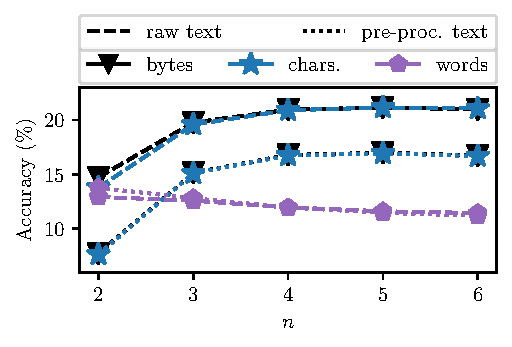
\includegraphics[
        width=\columnwidth,
        trim=0.8em 1.4em 0em 0em,
        clip
    ]{report/effect-of-n.pdf}
    \caption{Pre-processing and $n$ impact accuracy, SCAP, fixed $L=300$.}
    \label{fig:features}
\end{figure}

For brevity, we report only results from learners trained on these high
character $n$-grams and low word/flexible pattern $n$-grams.

% plot of SCAP accuracy vs. n for various levels, normalisation

\paragraph{Tuning hyper-parameters}

For each model, we tune our hyper-parameter using grid search
optimisation and the reduced training data, as follows:

We tune the profile length $L$ for SCAP using an 8-fold cross-validated
grid search over the reduced training data.

Evaluating each configuration of CNG, XRLP, and SRLP is more
computationally expensive, so for these models we tune $L$ using
holdout validation rather than 8-fold cross validation
(we train on 87.5\% of the reduced training data, and select the $L$
giving the highest accuracy on the other 12.5\%).

SPaCE models are our most computationally expensive to evaluate,
since smoothing removes the sparsity of profiles.
To tune the hyper-parameter for each smoothing method
($k$ for method i, $\alpha$ for method ii, and $K$ for method iii)
we perform a grid search using holdout validation on the reduced training
data, evaluating on 1000 tweets (0.3\%).
Due to time constraints, we only tune on character $n$-grams.

For our ensemble, we see the best results when combining
seven SCAP base models using character 2--6-grams,
word 2-grams, and flexible pattern 2-grams, respectively.


\paragraph{Model selection}
After turning each model/feature class combination using some 
partition(s) of the reduced training data, we re-train the
best-performing configurations on the entire reduced training set,
and evaluate their accuracy on our validation data.
We report the results in table \ref{tab:devresults}.




\begin{table}[h]
\centering
\begin{tabular}{@{}cccccccc@{}}
\cmidrule{3-8}
Acc. (\%)   &     & \multicolumn{6}{c}{Feature class}                    \\
\cmidrule{3-8} 
            &     & \multicolumn{3}{c}{character} & word  & \multicolumn{2}{c}{flex. patt.} \\
\cmidrule(r){1-1} \cmidrule(rl){3-5} \cmidrule(rl){6-6} \cmidrule(rl){7-8} 
Models      & $n$ & 4      & 5      & 6           & 2     & 2     & 3    \\
\cmidrule(r){1-1} \cmidrule{3-8} 
CNG         &     & 25.4   & 26.2   & 26.4        & 20.5  & 13.8  & 12.5 \\
SCAP        &     & 21.7   & 22.2   & 22.1        & 14.4  &  9.7  &  8.5 \\
XRLP        &     & 18.6   & 18.4   & 17.4        & 12.4  &  9.4  & 10.0 \\
SRLP        &     & 23.7   & 25.4   & 25.7        & 18.3  & 12.5  & 11.9 \\
SPaCE i     &     & 27.5   & 28.3   & 28.0        & ---   & ---   & ---  \\
SPaCE ii    & &{\bf 32.7}  & 32.2   & 30.9        & ---   & ---   & ---  \\
SPaCE iii   &     & 32.5   & 31.5   & 30.1        & ---   & ---   & ---  \\
                  \cmidrule{3-8} 
Ensemble    &     & \multicolumn{6}{c}{ ---23.4--- }\\ % (char23456grams+word2grams+flex2grams)
\bottomrule
\end{tabular}
\caption{Tuned model accuracy on held-out validation data.}
\label{tab:devresults}
\end{table}

We re-train our best performing model/feature class combination
(SPaCE ii, character 4-grams) on the entire labelled dataset for submission,
and achieve a public score of 34.7\%.

\section{Critical analysis}

% Should we spend any time discussing the tuning of individual hyperparameters?
    % L: too small and not enough broad information is captured in the profile, too large and it begins to capture noise as well (low counts are not reliable)
    % smoothing parameters: no smoothing is really bad. too much smoothing washes out all of the information in the distributions. duh?
% Should we say something about features, like the differences between words v. chars? v. bytes v. flexible patterns? How they work together in an ensemble?
    % flex patterns v. words: trading off structure/content. maybe in this dataset content is more reliable.
    % words v. chars: perhaps the lower density of words (fewer ngrams per tweet) exacerbates our lack-of-data-per-author problem, crippling these profile-baed methods (profiles are unreliable).
% Should we discuss the effect of normalisation? Or including a prior in some way? (we don't really have data for that)
% say something about models, why is simple RLP best local profile method?
% why is SPaCE so much better?
    % is it because we have so little data, so smoothing is critical, and truncation-based methods are 
    % is it because it corresponds to maximising the (log) likelihood of the tweet given the profile n-gram distributions as a generative model, with an independence assumption, even though that's naive?
    % an obvious tradeoff is that it's much slower than the other methods. Are the other methods 
% Why the heck does SRLP work at all?


% Compare local profile methods and compare to results found in literature - Alice
\paragraph{CNG v. SCAP v. RLP} Recent works show RLP out-performs CNG on large documents with few authors\supercite{layton2012recentred}, and SCAP out-performs CNG when there is limited training data per author\supercite{frantzeskou2006effective}. Our results show CNG outperforms both SCAP and RLP. We attribute these contrasting findings to how our dataset differs. RLP's measure of distinctiveness is less effective when there is limited training data per author because there is less data to compare distinctiveness. CNG and SCAP are comparative in performance until an authors profile becomes smaller than L\supercite{frantzeskou2006effective}. Our implementation overcomes this issue by padding an authors profile with unmatchable $n$-grams until it is at least L in length. This modification allows CNG to perform effectively on the dataset.

% compare character grams versus word and flex grams
% compare features. - Marvin
\paragraph{$n$-grams}
Previous work finds that $n=4$ for character $n$-grams is the most effective for Twitter data\supercite{layton2010authorship}, dropping in accuracy for $n<4$ and $n>4$. 
The study differs by using only few authors, around 50, whereas we have over 9,000. 
Our tests show that increasing $n$ tends to increase accuracy. 
Word and flexible pattern $n$-grams perform worse in isolation than character $n$-grams. % there's no talk on what word and flex actually represent about the text
While not the most effective alone, using a combination of these features simultaneously can improve accuracy\supercite{rocha2016authorship}.
However, the memory and time required to do so make it infeasible on any of our machines. 
% Character $n$-grams consistently outperform word and flexible pattern $n$-grams. 
% % Different levels of $n$-gram captures different information regarding an author's writing habits.
% Increasing $n$ for character $n$-grams tend to produce more accurate results (except in SPaCE).
% This contrasts studies which find that $n=4$ was the most effective parameter for their case\supercite{rocha2016authorship}. % actually it's from a citation in that citation which said n=4 is best
% The studies differ by having few authors - around 50 - whereas we have over 9,000. % IT'S OVER 9000!
% Combining the studies and our tests suggest that longer character $n$-grams are required as the number of authors increase.
% % Longer $n$-grams are potentially more specific to an author, as there is more variety of $n$-grams and less likely to be shared between authors.
% % However doing so also assumes that authors do repeat relatively long sections of text, otherwise learned $n$-grams will never appear in the test data. % learned? common? $n$-grams seen in training?
% % what do I say about words and flex
% Word $n$-grams performing consistently worse than character $n$-grams suggest that semantic information of a text is not as important as the raw information itself.
% % Longer character $n$-grams can in a sense substitute shorter word $n$-grams by capturing the $n$-grams that span multiple words while also capturing word uni-grams (1-gram).
% Flexible pattern $n$-grams performed the worse of all features.
% As it reflects the structure of a text rather than the contents, it may perform more effectively at longer texts. 
% However, our data comprises of texts with limited length, as such distinguishing structures may not emerge. 
% % However, with the given data we are dealing with the 140 character limit of a Tweet, there is not much room for distinguishing structure to emerge. % does that make sense? Do we need to justify why it didn't work?




% Combining the features in the ensemble performed better than word and flexible pattern by itself. Suggests ... orthogonal? - Shared
\paragraph{Ensemble} Char, word and flexible pattern $n$-grams are prone to error because of noise in the data. Combining the features in the ensemble model captures more information about authorship, suggesting that these features are orthogonal. An area of future work is to investigate more sophisticated methods to combine these features to build a more robust model. 
% suggests that independently each feature is prone to error (because noise?) but over multiple features the model is more robust? 

% yeah maybe think of it like: if everything about authorship that you could capture with word grams was already
% captured and utilised by the char models, then adding them together wouldn't help. it'd be like the information
% contained in the word models was a subset of the information in the character models.
% 'capture more information about authorship'? yeah that sounds about right
% ensemble is better -> it must capture more about authorship -> the features are orthogonal. -> future work investigate more elaborate ways to combine features (wraps it up nicely)
% that's perfect :) sweet thanks :)

% combining would  capture more information about authorship -> because features are orthogonal 
% minimise the errors is not quite the right phrase though
% hey what did you mean when the features are "orthogonal"?
% but the idea is that together  

% SPaCE is better than all profile methods. Why? - Matt
% \paragraph{SPaCE}
\paragraph{SPaCE} We observe that SPaCE models outperform all other models for
character-level $n$-grams.
Minimising $d_{space}$ corresponds to maximising
tweet (log) likelihood assuming tweets are sequences of
$n$-grams drawn independently from their author's $n$-gram
probability distribution.
It's somewhat surprising to see this level of performance,
given the naivety of this assumption.
However, SPaCE use a much richer profile representation
than other methods, with smoothing providing effective
regularisation. This may help it to make finer grained
distinctions between authors.

The choice of smoothing method is critical.
We see additive smoothing (i) outperformed by interpolation
smoothing (ii, iii).
Additive smoothing corresponds to assuming a uniform prior
on $n$-gram probability distributions when estimating profiles,
while interpolation methods take corpus-level frequency
information into account.
Since authors' $n$-gram distribution are indeed highly
non-uniform, interpolation smoothing is theoretically
more appropriate. % TODO: Reword this last sentence.
% If there's space (there's not),
% I might like to mention that we (I, at least) hypothesised
% method iii to be strongest, because empirical normalised frequencies
% should be more reliable than corpus information with more tweets
% for a but this was not the case empirically.

% Example citations of reviews \cite{rocha2016authorship, layton2010authorship, bhargava2013stylometric}, features from \textcite{schwartz2013authorship}, various models,\supercite{layton2012recentred, kevselj2003n, frantzeskou2006effective} and a tutorial\cite{layton2014tutorial}!

\printbibliography

\end{document}